\begin{figure}[t!]
    \centering
    \tikzstyle{every node}=[scale=0.80]
    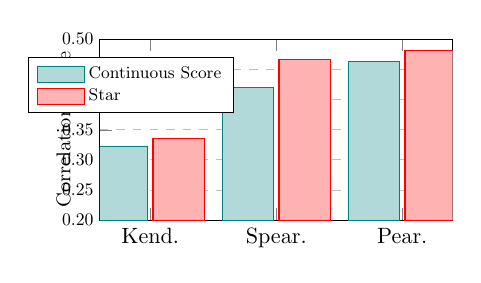
\begin{tikzpicture}
        \begin{axis}[
            ymajorgrids,
            grid style=dashed,
            at={(0,0)},
            width=.50\textwidth,
		  height=.32\textwidth,
            ybar,
            bar width=0.65cm,
            % enlargelimits=0.1,
            enlarge x limits=0.20,
            xtick=data,
            % xtick pos=bottom,
            xtick align=inside,
            nodes near coords align={vertical},
            ymin=0.20, ymax=0.50,
            ytick={0.20,0.25,...,0.50},
            y tick label style={scale=0.8,
                        /pgf/number format/fixed,
                        /pgf/number format/fixed zerofill,
                        /pgf/number format/precision=2},
            xticklabels={Kend., Spear., Pear.},
            ylabel={\small Correlation Score},
            ylabel style={yshift=-1.0em, scale=1},
            xlabel style={yshift=0.5em, scale=1},
            legend entries={\small Continuous Score, \small Star},
            % legend columns=2,
            % anchor=north,
            % nodes near coords,
            % nodes near coords style={font=\small},
            % nodes near coords style={/pgf/number format/.cd, fixed zerofill, precision=3},
            legend style={
                at={(0.38,0.9)},
                nodes={scale=0.85},
                legend cell align=left,
			  % legend plot pos=right,
                /tikz/every even column/.append style={column sep=0.10cm}},
            ]
            \addplot [fill=teal!30,draw=teal,area legend] coordinates {(1,0.322) (2,0.420) (3,0.463)};
                
            \addplot [fill=red!30,draw=red,area legend] coordinates {(1,0.336) (2,0.467) (3,0.481)};
          
        \end{axis} 
        \end{tikzpicture}
        \vspace{-2mm}
	\caption{
            The comparison of our CSEM with different prompt designs (star-based prompt and continuous score-based prompt).
        }
        \vspace{-2mm}
	\label{fig:star-score-compare}
\end{figure}